\section{Gapped Graphene}
The reason why the dispersion relation of graphene is degenerate in the $K$ points is due to the sub-lattice symmetry of the system. This means that for materials that don't have this symmetry such as Boron Nitrite exhibit an open gap in the $K$ points, alternatively one could layer graphene on top of another honeycomb lattice that doesn't have sublattice symmetry, therefore subjecting it with a periodic potential that breaks the symmetry and opens the gap.

Mathematically speaking, the tight binding Hamiltonian has two different energies for the two different atoms in the sub-lattice. With respect to equation \ref{eq:dirac_Hamiltonian} it becomes
\begin{equation}
    H_{\vect K_0}(\vect k)=
    -H^*_{\vect K_1}(\vect k)=
    \begin{bmatrix}
        \Delta& v_F\hbar(k_x-ik_y)\\
        v_F\hbar(k_x+ik_y)&-\Delta
    \end{bmatrix}
    \label{eq:gapped-dirac}
\end{equation}
Where $\Delta$ is half the difference of the diagonal energy on the two sublattices, and the energy zero has been shifted at the center of the energy gap. The dispersion relation now becomes
\begin{equation}
    E(\vect k)=\pm\sqrt{\Delta^2 + (v_F\hbar k)^2}
\end{equation}
It is seen that the above dispersion curves are formally the same produced by the Dira equations, with the light velocity $c$ replaced by the Fermi velocity $v_F$ and the rest mass $m_0=\Delta/v_F^2$

\begin{figure}[h]
    \makebox[\textwidth][c]{
        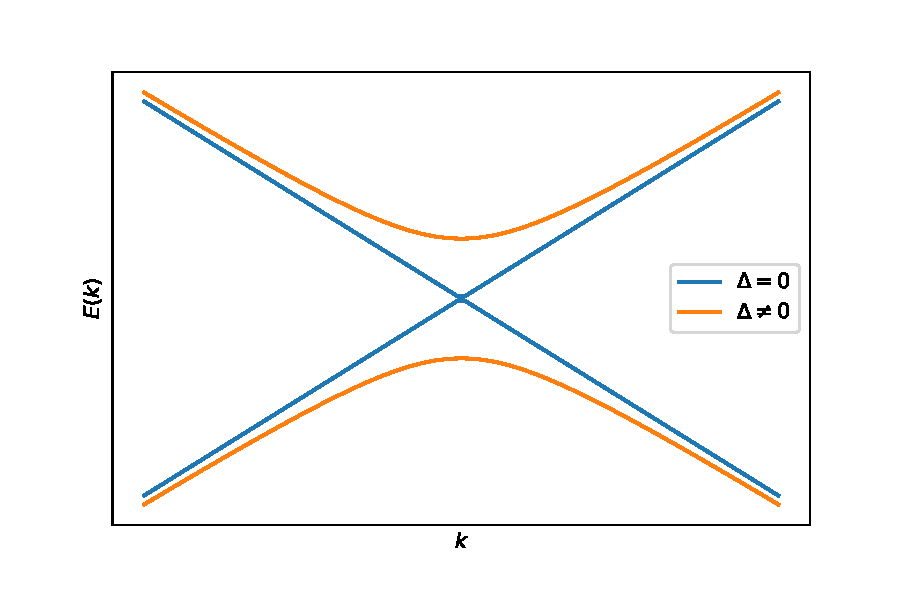
\includegraphics[width=\linewidth]{Immagini/graphene/dirac.pdf}
        }%
    \caption{difference between the gapless and the gapped Dirac dispersion relation}
    \label{fig:asd}
\end{figure}